\par Le membre en charge de cette partie était Antoine Pietri.

\par Les seuls obstacles que nous avons implémenté dans le jeu sont les trous noirs.
\par Nous nous sommes peu à peu rendu compte que ces obstacles encombraient trop le jeu et n'avaient
que peu d'utilité, c'est pourquoi nous avons décidé de ne pas en rajouter.
\par Les trous noirs sont des objets assez complexes puisqu'ils attirent le joueur en leurs centres en les faisant
tourner, ce qui a nécessité une bonne utilisation de nos connaissances en cinématique.

\begin{center}
	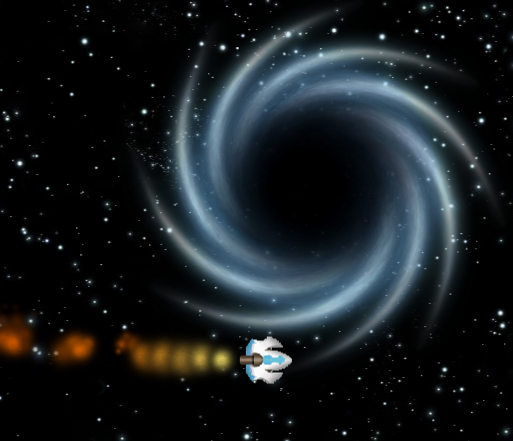
\includegraphics[width=260pt]{images/blackhole.png}
\end{center}

\par Leur but est donc d'attirer puis de bloquer le joueur en leurs centres. Pour cela nous procédons ainsi :
\begin{itemize}
	\item On commence par passer en coordonnées polaires dans un repère centré sur l'obstacle :
	$$ X_a = X_{vaisseau} - X_{obstacle} $$
	$$ Y_a = Y_{vaisseau} - Y_{obstacle} $$
	$$ R = \sqrt{X_a^2 + Y_a^2} $$
	$$ \theta = arctan(Y_a / X_a) $$
	
	\item On modifie $r$ et $\theta$ pour faire l'effet d'une spirale, on retourne en cartésien, puis on retourne dans le repère d'origine :
	$$X_{vaisseau} = (r - \Delta t \frac{G}{r^2}) \times cos(\theta - \Delta t \frac{\phi}{r^2}) + X_{obstacle}$$
	$$Y_{vaisseau} = (r - \Delta t \frac{G}{r^2}) \times sin(\theta - \Delta t \frac{\phi}{r^2}) + Y_{obstacle}$$
	avec $\phi$ et $G$ constantes (dans le jeu respectivement 1000 et 30), et $\Delta t$ le temps écoulé en secondes.
\end{itemize}